\PassOptionsToPackage{table}{xcolor}
\documentclass[9pt,xcolor=x11names,compress]{beamer}

%% General document %%%%%%%%%%%%%%%%%%%%%%%%%%%%%%%%%%
\usepackage{graphicx}
\usepackage{tikz}
\usetikzlibrary{decorations.fractals,lindenmayersystems}
\usepackage{wasysym}
%%%%%%%%%%%%%%%%%%%%%%%%%%%%%%%%%%%%%%%%%%%%%%%%%%%%%%


%% Beamer Layout %%%%%%%%%%%%%%%%%%%%%%%%%%%%%%%%%%
\useoutertheme[subsection=false,shadow]{miniframes}
\useinnertheme{default}
\usefonttheme{serif}
\usepackage{palatino}

\setbeamerfont{title like}{shape=\scshape}
\setbeamerfont{frametitle}{shape=\scshape}

\setbeamercolor*{lower separation line head}{bg=DeepSkyBlue4} 
\setbeamercolor*{normal text}{fg=black,bg=white} 
\setbeamercolor*{alerted text}{fg=DeepSkyBlue4} 
\setbeamercolor*{example text}{fg=black} 
\setbeamercolor*{structure}{fg=black} 
 
\setbeamercolor*{palette tertiary}{fg=black,bg=black!10} 
\setbeamercolor*{palette quaternary}{fg=black,bg=black!10} 

\setbeamertemplate{blocks}[rounded][shadow=true]
\setbeamercolor{block title}{bg=DeepSkyBlue4}
\setbeamercolor{block title example}{bg=DeepSkyBlue4}
\setbeamercolor{block body}{bg=black!15!white}
\setbeamercolor{block body example}{bg=black!15!white}

\setbeamertemplate{navigation symbols}{}
%%%%%%%%%%%%%%%%%%%%%%%%%%%%%%%%%%%%%%%%%%%%%%%%%%

\title{Lesson 1: Introduction to Functions}
\author[Francisco Blanco-Silva]{Francisco Blanco-Silva}
\institute[USC]{University of South Carolina}
\date{
\pgfdeclarelindenmayersystem{testrhombus}{
	\rule{F -> F+FF++FF+F+++F++F+++F}
}
\begin{tikzpicture}[color=DeepSkyBlue4]
    \draw [l-system={testrhombus, axiom=F+FF++FF+F+++F++F+++F, order=3, step=1.5pt, angle=90}]
    lindenmayer system; 
	\end{tikzpicture}	
}

\begin{document}
\frame{\titlepage}

\section{What do we know?}
\subsection{}

\begin{frame}\frametitle{What do we \alert{need to} know?}
    
\begin{itemize}
\item A solid background in High-School Algebra:
\begin{itemize}
	\item Simplifying Expressions
	\item Solving Linear Equations \alert{and Inequalities}
	\item Lines (and their graphs)
	\item Solving Quadratic Equations
	\item Quadratics (and their graphs)
	\item \alert{Logarithmic and Exponential Equations}
	\item Functions
	\begin{itemize}
		\item Evaluation
		\item Combination | Transformation
	\end{itemize}
\end{itemize}
\item It helps if you have been exposed to:
\begin{itemize}
	\item Polynomials
	\item Exponents | Powers
	\item \alert{Problem Solving}
\end{itemize}
\end{itemize}
\end{frame}

\subsection{}
\begin{frame}[c]\frametitle{Warm-up}
    
\framesubtitle{Lines: slopes, intercepts, \dots}

\begin{columns}

\begin{column}{0.5\linewidth}
\begin{block}
{A line can be defined by:}
\begin{itemize}
	\item \textcolor{red}{Two points $(x_1, y_1)$ and $(x_2, y_2)$.}
	\item A \textcolor{red}{point $(x_1, y_1)$} and slope $m$.
	\item Slope $m$ and \textcolor{blue}{$y$-intercept $a$}.
\end{itemize}
\end{block}
\end{column}

\begin{column}{0.5\linewidth}
\begin{center}
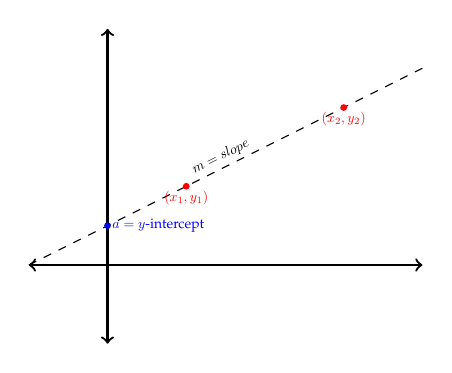
\begin{tikzpicture}
\draw [thick, <->] (0, -1) -- (0, 3);
\draw [thick, <->] (-1, 0) -- (4, 0);
\draw [dashed] (-1, 0) -- (4, 2.5) node [midway, sloped, above, scale=.5] {$m = \text{slope}$};
\filldraw [red] (1, 1) circle (1pt) node [scale=0.5, below] {$(x_1, y_1)$};
\filldraw [red] (3, 2) circle (1pt) node [scale=0.5, below] {$(x_2, y_2)$};
\filldraw [blue] (0, .5) circle (1pt) node [scale=0.5, right] {$a = y$-intercept};
\end{tikzpicture}
\end{center}
\end{column}
\end{columns}

\begin{align*}
	\uncover<2->{y - y_1 &= \frac{y_2 - y_1}{x_2 - x_1} (x - x_1) & \big(\text{slope} &= \frac{y_2 -y_1}{x_2 - x_1} = \frac{y_1 - y_2}{x_1 - x_2} \big)  \\}
	\uncover<3->{y - y_1 &= m (x-x_1)\\}
	\uncover<4->{y &= a + m x}
\end{align*}

\end{frame}

\section{Functions: A Review}
\subsection{}

\begin{frame}[c]\frametitle{Functions}
    
\framesubtitle{Definition and Representation}

\begin{definition}
A \alert{function} is a rule that takes certain numbers as inputs and assigns to each a definite output number.

\pause The set of all input numbers is called the \alert{domain} of the function, and the set of resulting output numbers is called the \alert{range} of the function.
\end{definition}

\pause
\begin{center}
\rowcolors{2}{white}{gray!50!white}
	\begin{tabular}{c||c}	
		\rowcolor{DeepSkyBlue4}	
		 & a.k.a. \\
		input & \alert{independent variable} \\
		output & \alert{dependent variable} \\
		range & \alert{image}
	\end{tabular}
\end{center}

\pause

\begin{columns}
\begin{column}{.5\linewidth}
Functions can be represented:
\begin{itemize}
	\item \alert<5>{By tables}
	\item \alert<6>{By graphs}
	\item \alert<7>{By formulas}
	\item \alert<8>{With word descriptions}
\end{itemize}
\end{column}
\begin{column}{0.5\linewidth}
\only<5>{\includegraphics[width=0.6\linewidth]{weather.png}}
\only<6>{\includegraphics[width=0.7\linewidth]{ekg.png}}
\only<7>{
	\begin{equation*}
		A = \pi r^2
	\end{equation*}
}
\only<8>{
	
	The area of a circle is $\pi$ times the square of its radius.
}
\end{column}
\end{columns}
\end{frame}

\begin{frame}[c]\frametitle{Functions}
    
\framesubtitle{Examples}

We write $y = f(t)$ to express that $y$ (\alert{the dependent variable}) is a function of $t$ (\alert{the independent variable}).

\begin{example}
\alert{The value of a car in thousands of dollars, $V$, is a function of the age of the car, $a$, in years.}
\begin{equation*}
\alert{V = f(a)}
\end{equation*}
\begin{itemize}
	\item \alert{What is the independent variable? And the dependent variable?}

	\pause Independent variable: age of the car, $a$, in years

	\pause Dependent variable: value of the car, $V$, in thousands of dollars
	\item<4-> \alert{What does it mean $f(5)=9$?}

	\pause\pause 
	After five years, the car is worth \$9,000.
\end{itemize}
\end{example}
\end{frame}

\begin{frame}[c]\frametitle{Functions}
    
\framesubtitle{Examples}

\begin{example}
\alert{The value of a Honda Civic is approximated by $V = f(a) = 13.78 - 0.8a$:}
	\begin{itemize}
		\item \alert{What is the significance of $f(0)$?}
		\pause
			\begin{equation*}
			f(0) = 13.78 - 0.8 \times 0 = 13.78
			\end{equation*}

		The value of a brand new Honda Civic is about \$13,780.

		\item<3-> \alert{For what value of $a$ is $f(a)=0$?  What is the significance of this $a$-value?}
		\begin{align*}
		\uncover<4->{f(a) &= 0 \\}
		\uncover<5->{13.78  - 0.8a &= 0 \\}
		\uncover<6->{13.78 &= 0.8 a \\}
		\uncover<7->{a &= \frac{13.78}{0.8} \approx 17.22}
		\end{align*}
		\pause\pause\pause\pause\pause\pause
		In about 17 years, this car will be worthless!
	\end{itemize}
\end{example}
\end{frame}
\end{document}